\section{断熱パイプラインの熱伝達}
この例では、断熱されたパイプラインに熱負荷がかかります。その寸法は:
\begin{itemize}
\item 外径:57 mm
\item 内径: 50 mm
\item 断熱材の厚さ: 28 mm
\item 長さ: 200 mm
\end{itemize}
\begin{enumerate}
\item
  {[}mm, ton, s, °C{]}単位の新規ファイルを作成し、ステップ形式のジオメトリをPrePoMaxにインポートします。
  次に、両方のパーツをメッシュ分割します。
  ここでは、最大要素サイズとして、断熱材は2mm、パイプは3mmを選択しました。その他の設定は変更しませんでした(図\ref{fig:11-01})。
	\begin{figure}[H]
	\centering
	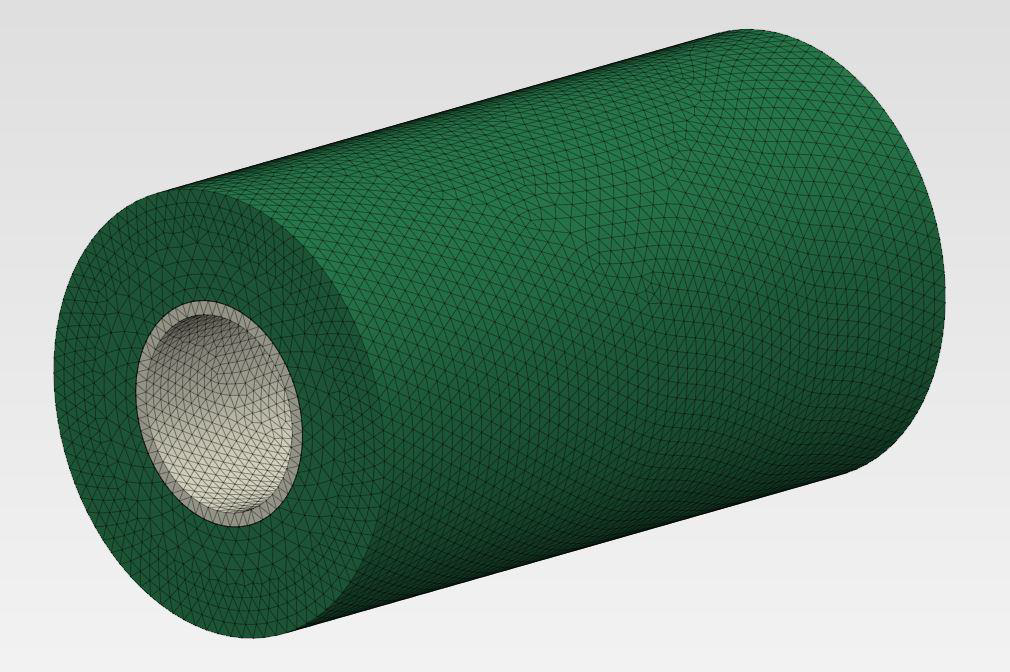
\includegraphics[width=125mm]{fig/11-01.png}
	\caption{パイプライン - メッシュ}
	\label{fig:11-01}
	\end{figure}
	\vspace{-\baselineskip}
\item
  Pipe\_materialという名前の新しいマテリアルを定義し、Thermal conductivity(熱伝導率)を追加して、45mW/(mm-°C)という値を指定します。
  もう1つのマテリアルを定義し、名前をInsulation\_materialとし、Thermal conductivity(熱伝導率)を追加して値を0.05mW/(mm-°C)とします。
  Pipe\_materialを材料として、Pipe\_sectionという名前のソリッドセクションを新規に作成し、そのセクションが割り当てられるように内側のパーツ(パイプ)を選択します。
  別のセクションを作成し、名前をInsulation\_sectionとし、マテリアルとしてInsulation\_materialを選択し、外側のパーツ(断熱材)を選択します。
\item
  パイプを非表示にして、断熱材の内側の面にTie1という名前のサーフェスを作成します。パーツの可視性を反転させ(View → Invert Visible Parts)、パイプの外側の面にTie2という名前のサーフェスを作成します。
  再び両方のパーツを表示します。
  タイ拘束を定義し、以前に作成したサーフェスをマスターとスレーブ領域として使用します。
\item
  熱伝導解析ステップをデフォルト設定(定常状態)で定義します。
\item
  Convective film loadを作成し、断熱材の外表面に割り当てます。
  シンク温度を20°C、熱伝達率を0.015 mW /(mm2・°C)に指定します。
  Convective film loadをもう1つ作成し、パイプの内側表面に割り当てます。
  シンク温度は-30℃、熱伝達率は0.8mW/(mm2-°C)に指定します(図\ref{fig:11-02})。
  	\vspace{-.3\baselineskip}
	\begin{figure}[H]
	\centering
	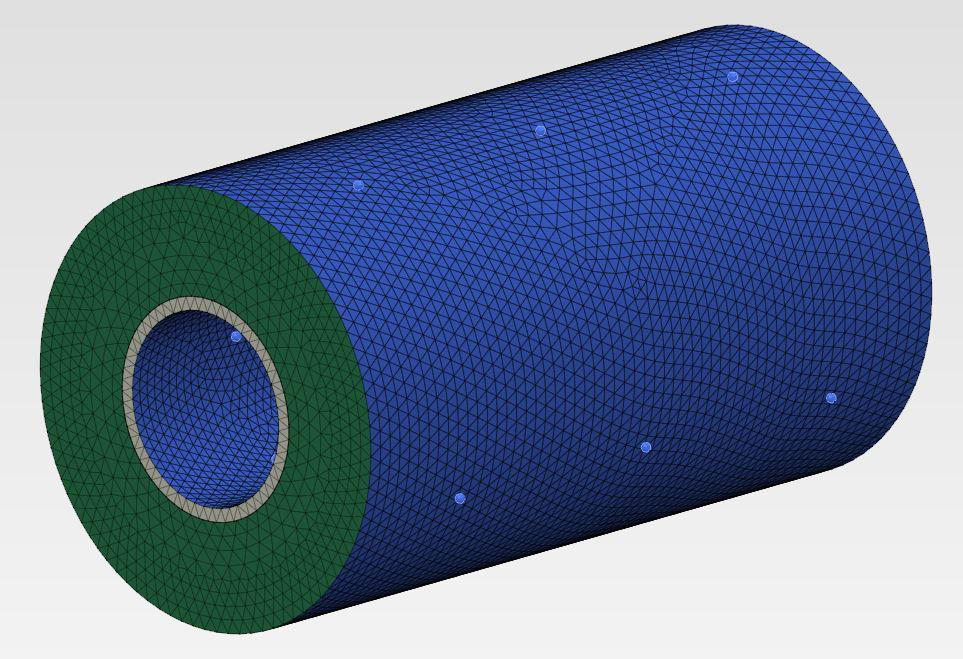
\includegraphics[width=104mm]{fig/11-02.png}
	\caption{パイプライン - 熱負荷}
	\label{fig:11-02}
	\end{figure}
	\vspace{-\baselineskip}
\item
  必要な定義がすべて行われたので、解析を提出できます。
  解析が終了するまで待って、結果を開きます。
\item
  温度コンタープロットを調べます(図\ref{fig:11-03})。
  分析的に計算されたパイプの内側の面の温度は-29.83℃で、パイプの外側の面の温度は16.05℃です。
  同様の値は解析でも確認できます(Query toolで確認してください)。
  	\vspace{-.3\baselineskip}
	\begin{figure}[H]
	\centering
	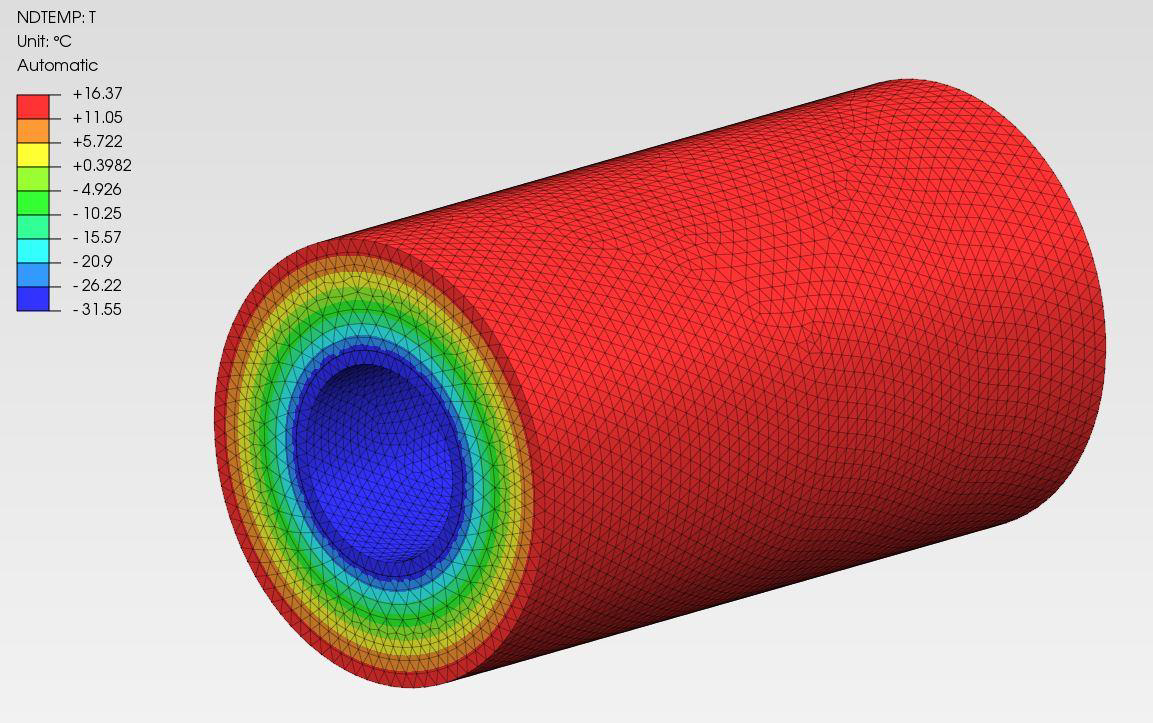
\includegraphics[width=128mm]{fig/11-03.png}
	\caption{パイプライン - 温度}
	\label{fig:11-03}
	\end{figure}
	\vspace{-\baselineskip}
\end{enumerate}